This note describes a search for the associated production of a Higgs boson and a single top quark, events with two same-sign leptons or three leptons, targeting Higgs decay modes to $\PW\PW$, $\Z\Z$, and $\Pgt\Pgt$.
The analysis uses the 13\TeV\ dataset produced in 2016, corresponding to an integrated luminosity of 35.9\fbinv.
It is based on and expands previous analyses at 8\TeV~\cite{Khachatryan:2015ota,CMS_AN_2014-140} and searches for associated production of \ttbar\ and Higgs in the same channels~\cite{CMS_AN_2016-211}, and complements searches in other decay channels targeting $\PH\to\cPqb\cPaqb$~\cite{CMS_PAS_HIG_16-019}.

The production cross section of the single top plus Higgs boson (\tHq) process is driven by a destructive interference of two main diagrams (see Fig.~\ref{fig:thq_prod}), where the Higgs couples to either the \PW\ boson or the top quark.
Any deviation from the standard model (SM) in the Higgs coupling structure could therefore lead to a large enhancement of the cross section, making the analysis sensitive to such deviations.
A second process, where the Higgs and top quark are accompanied by a \PW\ boson (\tHW) has similar behavior, albeit with a weaker interference pattern.

\begin{figure}[!htb]
\begin{center}
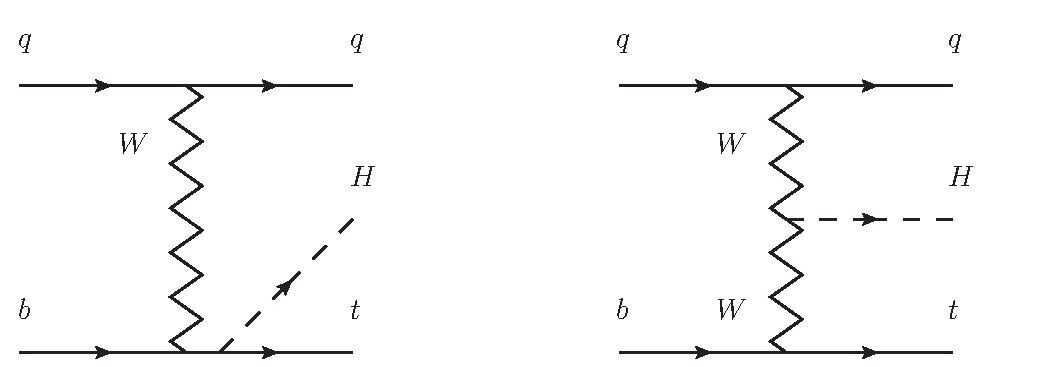
\includegraphics[scale=0.7]{figures/qtH.pdf}
\end{center}
\caption{The two leading-order diagrams of \tHq\ production.}
\label{fig:thq_prod}
\end{figure}

The analysis selects events with either a pair of leptons of equal charge, or with three leptons, as well as \cPqb\ tagged jets.
The \tHq\ signal contribution is then determined in a fit of the observed data to two multivariate classifier outputs, each trained to discriminate against one of the two dominant backgrounds of events with non-prompt leptons from \ttbar\ and of associated production of \ttbar\ and vector bosons (\ttW, \ttZ).
The fit result is then used to set an upper limit on the combined \tHq\ and \tHW\ production cross section, as a function of the relative coupling strengths of Higgs and top quark and Higgs and \PW\ boson, respectively.

\paragraph*{Related presentations in CMS meetings}
\begin{itemize}
	\item[-] Top Higgs Forum, Hamed~Bakhshiansohi, Sep.~13$^{rd}$, 2016 \hfill{\small \href{https://indico.cern.ch/event/567994/}{\textcolor{blue}{agenda}}}
	\item[-] HWW Meeting, Jose~Monroy, Oct.~19$^{th}$, 2016 \hfill{\small \href{https://indico.cern.ch/event/566851/#b-225107-higgs-to-ww}{\textcolor{blue}{agenda}}}
	\item[-] HWW Meeting, Jose~Monroy, Dec.~14$^{th}$, 2016 \hfill{\small \href{https://indico.cern.ch/event/566859/#b-225187-higgs-to-ww}{\textcolor{blue}{agenda}}}
	\item[-] HWW Meeting, Pallabi~Das, Dec.~16$^{th}$, 2016 \hfill{\small \href{https://indico.cern.ch/event/566826/#b-235251-hwwwwleptons-cross-in}{\textcolor{blue}{agenda}}}
	\item[-] ttH Leptonic Meeting, Pallabi~Das, Jan.~19$^{th}$, 2017 \hfill{\small \href{https://indico.cern.ch/event/598405/?filterActive=1&showDate=all&showSession=16}{\textcolor{blue}{agenda}}}
	\item[-] Pre-approval, Jose~Monroy, Feb.~7$^{th}$, 2017 \hfill{\small \href{https://indico.cern.ch/event/605481/#b-240093-higgs-meeting-moriond}{\textcolor{blue}{agenda}}}
\end{itemize}
